\newpage
\chapter{Literature Review}
\label{Literature}

\lhead{\emph{Literature Review}} % Set the left side page header to "Symbols"

In this chapter we explore previous results, as well as introducing relevant concepts.




\section{Condorcet Domain}
If our goal is to prevent Condorcet cycles, or in general have transitive majority relations, the best we could hope to do is to apply our domain restriction such that our domain contains all profiles $P$ such that $P$ has a (weak) Condorcet winner. We call this domain $\domain{Condorcet}$. Under this domain, let $\votingrule{Condorcet}$ be the Condorcet Rule, which picks a Condorcet winner. Then $\votingrule{Condorcet}$ is strategyproof over $\domain{Condorcet}$ \citep{elkindPreferenceRestrictionsComputational2022}.

\begin{proofc}{(\citet{elkindPreferenceRestrictionsComputational2022})}.
	Assume, for the sake of a contradiction, we have profiles $\strictProfile = (\pref_1 \dots \pref_i \dots \pref_n)$ and $\strictProfile' = (\pref_1 \dots \pref_{i'} \dots \pref_n)$ such that:
	\[
		\votingrule{Condorcet}(P) = a, \quad \votingrule{Condorcet}(P') = b, \quad \text{and } a \neq b
	\]
	Assume that $i$ has $b \pref_i a$, then under $\strictProfile$ a strict majority $N' \subseteq N$ have $a \pref b$, but $i \notin N'$, thus in $P'$, $N'$ is still a majority preferring $a$ to $b$, but this is in contradiction to $b$ winning in $P'$.
\end{proofc}

This result is strengthened by \citet{campbellNonmonotonicityDoesNot2002,campbellCorrectionStrategyproofnessCharacterization2016}, showing that for an odd number of candidates, \(f_{\text{Condorcet}}\) is the only voting rule over \(\domain{Condorcet}\) that is Strategyproof, Surjective and Non-dictatorial.

When Surjectivity is strengthened to Neutrality, and Non-dictorship to Anonymity, \linebreak \(f_{\text{Condorcet}}\) is the only Strategyproof voting rule over \(\domain{Condorcet}\) for an odd number of voters \cite{campbellAnonymousNeutralStrategyproof2015}.

\subsection{Hereditary Domains}

Though this result is positive, we might wonder how stable it is, for this we need to define a notion of stability. On natural way to think about it is as follows: suppose one of the candidates or voters drops out, do we keep the nice structure of the domain? If this is true we call a domain \emph{Hereditary}.

\begin{definition}{Hereditary \textnormal{(\citet{elkindPreferenceRestrictionsComputational2022})}}{dom-hereditary}
	A domain restriction onto $\domain{ }$ is \emph{hereditary} if, for every profile $P \in \domain{ }$, and every profile $P'$, that can be obtained by deleting voters and candidates from $P$, $P'$ is also in $\domain{ }$
\end{definition}

$\domain{Condorcet}$ is not hereditary, this is easy to see through an example:

\begin{example}{$\domain{Condorcet}$ is not hereditary}{con-her}
	\begin{minipage}{0.25\linewidth}
		\begin{tabular}{cccc}
			\toprule
			$v_1$ & $v_2$ & $v_3$ & $v_4$ \\
			\midrule
			$a$   & $b$   & $c$   & $a$   \\
			$b$   & $c$   & $a$   & $c$   \\
			$c$   & $a$   & $b$   & $b$   \\
			\bottomrule
		\end{tabular}
	\end{minipage}
	\begin{minipage}[b]{0.70\linewidth}
		We can see that in this example, $a$ is the weak Condorcet winner, as it beats $b$ and is tied with $c$, however if we remove voter 4, we return to the original Condorcet cycle.
	\end{minipage}
\end{example}

A domain not being hereditary means that the nice properties of the domain can be unstable, as the number of voters and candidates might not be known or could be manipulated. Instead, we might want to look at hereditary domains. We present the single-peaked domain, will also be the main focus of this thesis. This is the domain of all single-peaked profiles.


\begin{proposition}{\textnormal{(\citet{elkindPreferenceRestrictionsComputational2022}).}}
	$\domain{SP}$ is hereditary.
\end{proposition}

\begin{proofc}
	(Voter Deletion). If we remove a voter, this does not affect the other voters, thus the profile is still single-peaked.~\checkmark

	(candidate Deletion). Consider any voter $i$ and their single-peaked vote, if we remove some candidate $x$, to this voter all candidates which voter $i$ preferred to $x$ stay in the same position, while all other candidates move up one rank, thus preserving the order, and single-peakedness.~\checkmark
\end{proofc}

% A similar notion to single-peaked profiles is that of single caved profiles, which is equivalent, but instead of a voters peak representing their most preferred option, they have a valley, which represents the worst option. Single caved profile are hereditary as well, but for a voting rule on them to be strategy proof, only two possible candidates can be chosen, the left and right most candidates according to $\orderalt$.

% Instead of ordering the candidates, we can imagine instead ordering the voters, such that we have a leftmost and rightmost voter, and all other voters can be placed between them based on their difference. In this case, a profile is single-crossing if, for any candidate $a$, its preference relation to another any candidate $b$ flips at most once when traversing the voters in order $\orderalt$.
%
% \begin{definition}{Single-Crossing Profiles \textnormal{(\citet{elkindPreferenceRestrictionsComputational2022})}}{single-crossing}
% 	A profile $P$ is single-crossing w.r.t. some ordering $\orderalt$, if for any $a,b \in X$, $\{i \in N : a \pref b\}$ and $\{i \in N: b \pref_{i} a\}$ are both intervals over $[n]$. A profile $P$ is single crossing if the votes can be permuted such that it is single crossing w.r.t. some ordering.
% \end{definition}
%
% Similar to single-peaked profiles, the domain of single-crossing profiles, $\domain{SC}$ is also hereditary
%
% \begin{proposition}
% 	$\domain{SC}$ is hereditary
% \end{proposition}
%
% \begin{proofc}
% 	(Voter Deletion). Deleting a voter preserves the ordering between voters, as such this cannot introduce a new crossing between candidates.~\checkmark
%
% 	(candidate Deletion). If we remove an candidate, the voters' rankings of the other candidates does not change, thus preserving single-crossing.~\checkmark
% \end{proofc}

As the goal is to ensure we find ourselves in nicely structured domains, we
need some mechanism through which we can ensure this is the case. Deliberation
is one possible pathway towards this. We will now provide a brief overview of the
literature surrounding deliberation.

\section{The History of Deliberation and Meta-Agreement}

We have provided an overview of different domain restrictions and their
properties, showing they avoid Condorcet cycles.
\citet{bochslerMarquisCondorcetGoes2010} argue however, that Condorcet cycles
are empirically rare. The next section is dedicated to explaining how
deliberation might explain this is so through examining the historical ideas
around deliberation and deliberative democracy, as well as that of
Meta-Agreement.

\subsection{Deliberation}

Though deliberation is intuitively familiar, namely
the process of multiple people talking through a problem with the goal of
coming to an agreement, compromise or solution. Providing a definition that is
both clear and consistent with the literature in Political Science, Philosophy
and Social choice is difficult.  As this intuition leaves some of the reasons for
and goals of deliberation, as stated in the literature, unmentioned.


% !TODO Explain how deliberative democracy is even related to deliberation

\citet{freemanDeliberativeDemocracySympathetic2000} gives an overview of deliberative democracy, in which he shares the intuitive idea that a deliberative democracy contains open discussion, open legislative deliberation and a pursuit of the common good. He also notes that there is no common agreement on the central features of a deliberative democracy, one account is that of deliberative democracy simply involving discussion among the public before voting. Another similar account is that this voting must not only be preceded by deliberation, but also general communication, all of which intended to change people's preferences. He further proceeds to give a more detailed conception of deliberative democracy, according to which a deliberative democracy is one in which political agents or their representatives

\begin{enumerate}
	\label{list:deliberative-democracy}
	\setlength\itemsep{1px}
	\item  Aim to collect, deliberate and vote
	\item  Represent their sincere and informed judgements
	\item  Vote and deliberate on measures beneficial to the common good on the citizens
	\item  Are seen and see each other as political equals
	\item  Have Constitutional rights and their social means enable them to participate in public life
	\item  Are individually free, such that they have their own freely determined conceptions of the good
	\item  Have diverse and disagreeing conceptions of the good
	\item  Recognize and accept their duty as democratic citizens, and do not engage in public argument on the basis of their particular moral views incompatible with public reason.
	\item  Agree reason is public, in so much as it is related to and advances common interests of citizens
	\item  Agree that their common interest lies primarily in freedom, independence and equal status as citizens.
\end{enumerate}

\textcolor{OrangeRed}{Firstly, why suddenly talk about deliberative democracy? how is this different from deliberation. Secondly, does this imply that this is already the case? Or should we aim to achieve a deliberative democracy?}

These features allow us to be more precise when we talk about a deliberative democracy, and in turn be more careful about what deliberation must entail. \citet{cohenDeliberationDemocraticLegimitimacy2002} further argues that deliberation is needed for democratic legitimacy. By this he means that without deliberation, a democracy is simply the will of the majority, but since majority rule is unstable, it is simply a reflection of the particular institutional constrains at the time. He further goes on to describe the \emph{ideal deliberative procedure} as follows

\textcolor{OrangeRed}{What does it mean to be unstable in this context? Elaborate on "particular institutional constraints"}

\begin{enumerate}
	\label{list:ideal-deliberation}
	\setlength\itemsep{1px}
	\item  Ideal deliberation is \emph{free}, participants regard themselves as only bound by the results of the deliberation, and the preconditions thereof. Participants act in accordance with the decision made through deliberation, and it being agreed on is sufficient reason to do so.
	\item  Ideal deliberation is \emph{reasoned}, parties are required to state their reasons for advancing proposals.
	\item  In ideal deliberation, parties are \emph{equal}, both formally and substantively. There are no rules that single individuals out, and existing distributions of power to no lend a party the opportunity to contribute to deliberation.
	\item  Ideal deliberation aims to arrive at \emph{consensus}, which can be rationally defended.
\end{enumerate}

\subsection{Meta-Agreement}
\label{subsection:Meta-agreement}

Consensus, sometimes referred to as substantive agreement, then seems like a
natural goal for deliberation. \citet{elsterMARKETFORUMThree2002} argues that
this is not only the goal, but through unanimous agreement this process
completely replaces voting, thereby circumventing Arrow's impossibility
theorem: ``Or rather, there would not be any need for an aggregation mechanism,
since a rational discussion would tend to produce unanimous preferences.'' (p.
112). Though it would be desirable to circumvent Arrow's impossibility theorem,
in practice people, even after deliberation, might not and indeed often do not
come to full substantive agreement. \citet{listTwoConceptsAgreement2002}
instead proposes another perspective  on deliberation based on Meta-Agreement

Under \emph{Meta-agreement} individuals do not need to agree on their most
preferred outcome, instead they only need to agree on the dimensions of the
problem. To contrast this with Substantive-agreement, under which individuals
do not need to conceive of the problem in the same way, all they need is to
agree on the same outcome. This means that under substantive agreement, voters
can agree outcome $a \pref b$ for different reasons, while under
Meta-Agreement, if voters disagree on $a \pref b$ it must be for the same
reason.

According to \citet{listTwoConceptsAgreement2002} there are three hypotheses that need to be satisfied for deliberation to induce meta-agreement:
\begin{enumerate}
	\label{list:meta-agreement-checklist}
	\setlength\itemsep{1px}
	\item [D1] Deliberation leads people to discover a single \emph{issue}-dimension
	\item [D2] Deliberation lets people place all possible candidates in this \emph{issue}-dimension
	\item [D3] After this deliberation, people update their preferences by picking
	      a preferred outcome, and all other rankings are based on the distance to this outcome in the \emph{issue}-dimension
\end{enumerate}

All these are necessary conditions for \emph{meta-agreement}, from this is it
also clear to see that, given that there is exactly 1 \emph{issue}-dimension,
single-peaked profiles are, by definition, a direct consequence. This is the
main reason meta-agreement is desirable, as it lets us circumvent the
Gibbard-Satterthwaite theorem \citep{gibbardManipulationVotingSchemes1973,
	satterthwaiteStrategyproofnessArrowsConditions1975} through restricting the
domain of preference profiles to the single-peaked domain $\domain{SP}$


\citet{listDeliberationSinglePeakednessPossibility2013} provide empirical
evidence for this theory of deliberation, showing deliberation increases
proximity to single-peakedness through voter deletion (PtS-V), which they define as $S= \frac{m}{n}$
where $n = |\voters|$ and $m$ is the largest subset of voters such that their
profile is single-peaked. Furthermore, they also introduce the notion of
salience, which represents to what extent a topic is salient in the voting
population. In order to test whether deliberation increases single-peakedness
\emph{through} meta-agreement, they test the following four hypotheses: (H1)
deliberation increases PtS-V. (H2')\footnote{This is a
	test for a corollary. H2 states that the rate of increase of PtS-V decreases. This is not experimentally testable, however since
	high salience means some sort of deliberation has happened before, they expect
	this to approximate this affect.} high salience issues show less increase in
PtS than low salience issues. (H3) Effective deliberation, in the sense that
more is learned during deliberation, results in bigger increases of PtS. (H4)
All things equal, the increase is largest for issues with natural
\emph{issue}-dimensions. They find support for all these hypothesis, showing
that on low-moderate salience issues PsT increases following deliberation.

It is important to note that these claims simply predict what will happen,
there is not much explanatory power to these claims. Little is known about to
process be which voters signal the issue dimensions, nor how they decide on
which ones to present.

\textcolor{OrangeRed}{TODO Read the paper again}
Furthermore,~\citet{ottonelliElusiveNotionMetaagreement2013} show
meta-agreement to be a stronger requirement than it may seem at a first glance.
Firstly for (D1) to hold, the \emph{issue}-dimension must hold some semantic
meaning, as it is unclear how people can exchange conceptualization
of the problem otherwise. Furthermore, the issues must consist of 2 semantic
issues, with only 1 issue voters simply reach substantive
agreement. A further restriction on these two dimensions is that they need to
be opposite, with opposite justifications. If this is not the case, a voter can
agree with both justifications, and thereby introduce a new dimension
``balance'', which then violates the conditions under which single-peaked
profiles guarantee the existence of fair, strategyproof voting rules. D2
requires that all voters share the exact same semantic understanding of the
dimension, and the outcome associated with each candidate. Finally D3
requires D1 and D2 to have happened before in order. D3 seems to be the easiest
hypothesis to satisfy.

Thus, meta-agreement as a means for single-peaked profiles is still quite
restrictive, needing multiple forms of unanimity, and only applying to problems
with certain properties. Nonetheless,  meta-agreement could still provide
explanatory power to deliberation.

\section{Models of Deliberation} \label{section:related_work} % work on this title
\citet{radDeliberationSinglePeakednessCoherent2021} model deliberation and its
effect on single-peakedness, though they argue single-plateauedness is a more
accurate term. To this end, they model deliberation as the process of all
voters announcing their preferences, and all other voters updating their
current preference towards that of the announced preference, in doing so they
might have a bias towards their own preference, as such they try to minimize
the distance between their current preference and the announced one. This
process repeats until all voters have announced their opinion once, which
constitutes one ``round'' of deliberation. The preference a voter adopts when
updating must lie between their current profile and the announced profile,
which profiles are considered to be ``between'' is defined by the distance
metric used. They considered three distance metrics, Kemeny-Snell
(KS)~\citep{kemeny1962preference}, Duddy-Piggins
(DP)~\citep{duddyMeasureDistanceJudgment2012}, and Cook-Seiford
(CS)~\citep{cookPriorityRankingConsensus1978}. Both KS and DP depend on the
judgement set resulting from the voters preferences, which is contains, for
each pair of candidates $a,b$, where $a \neq b$, a proposition $(a \pref b)$ or $\neg (a
	\pref b)$. The KS distance is then defined as the number of binary swaps a
judgement set needs to undergo before it becomes the target judgement set, an
example for such a swap would be going from $(a \pref b)$ to $\neg (a \pref
	b)$. The DP distance is defined on the graph of judgement sets, where 2 sets
share an edge if there is no judgement set between them. Since KS and DP share
their notion of betweenness, we introduce their betweenness as follows.

\begin{definition}{J-Betweenness}{def:j-between}

	A judgement set $J_i$ is between preferences $J_j$ and $J_k$ if for
	every $x,y \in \alternatives$, $J_i$ either agrees with the proposition
	in $J_j$ or $J_k$.

\end{definition}

From this definition it is clear that this could only result in a voter
updating their original opinion in which they have $(a \pref b)$ to a new
opinion where $\neg (a\pref b)$ only if the announced opinion contains $\neg (a
	\pref b)$.

\Cref{figure:DPDistance} shows a graph used for the DP distance in the case of
3 candidates, for simplicity the associated preferences are used to label the
judgement sets.


The CS distance is simpler and is simply defined as the number of positions two
voters disagree on, and a preference is between two others if for each position
it agrees with one of the two preferences.

Each distance has different trade-offs, CS is the simplest, but might
exaggerate the distance when there are many candidates, for example if 2
voters agree on the relative ranking of all but 1 candidate, which one voter
happens to rank first, thereby shifting the opinion of voter 2 right by one,
the CS distance would conclude that these voters are in full disagreement,
while reasonably one could conclude their opinions do not differ much. The KS
distance, using judgement sets instead of raw profiles captures this more
effectively, while still being relatively easy to compute, but in cases of more
disagreement, it is likely to over count the distance, since the binary changes
do not capture logical necessities. For example, swapping $( a \pref b)$ to
$\neg (a \pref b)$ must result in $(b \pref a)$ becoming true (in the case of
strict preferences), thus one might reasonably conclude this should only count
as 1 step. DP improves upon this, but in doing so becomes much harder to
compute, mainly through the cost of constructing the full graph of judgement
sets, which grows in $f_n = 1 + \sum_{j=1}^{n-1} \binom{n}{j} f_{n-j}$ in the
number of vertices, where $n$ is the number of candidates~\cite{grossPreferentialArrangements1962}. This can easily be
verified by noting that the number of judgements sets over $n$ corresponds to
the number of weak preference rankings over $n$ candidates, which is defined
as candidates, and a binary choice on each proposition.



\vspace{1em}
\begin{figure}[ht]
	\centering
	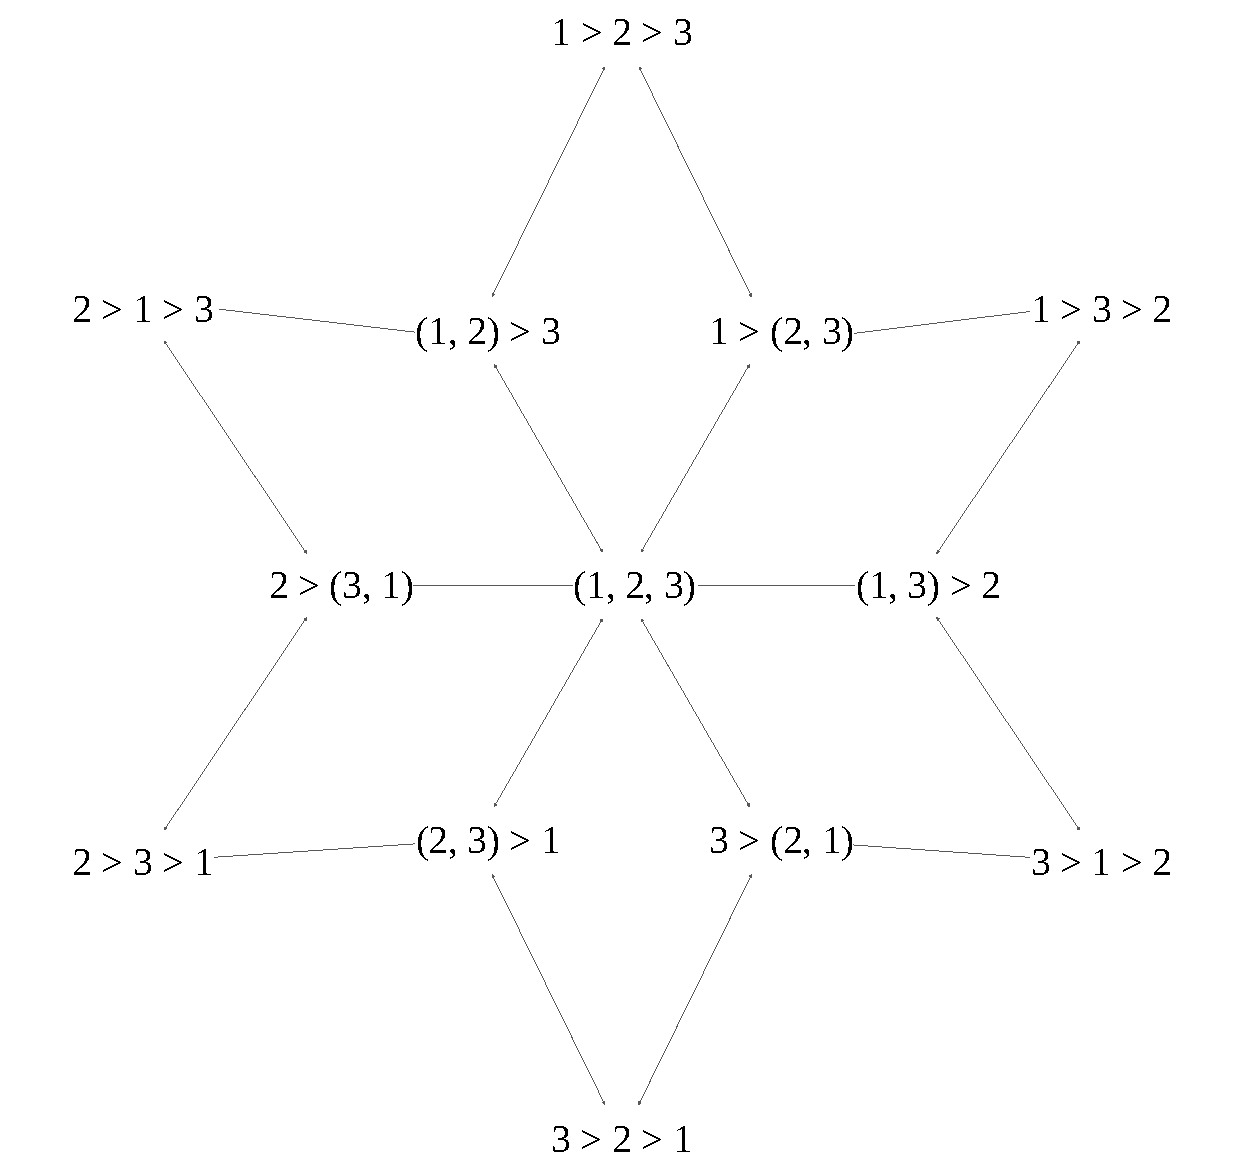
\includegraphics[width=0.65\textwidth]{dpGraph.pdf}
	\caption{The graph of judgement sets for all preferences over three candidates, brackets indicate ties.}
	\label{figure:DPDistance}
\end{figure}


% TODO D_s should be a map from the set of all possible voters with all possible r to the set of all voters
% TODO also clear up notation, d_s is the distance, D_s notation? this is messy
Apart from these distances, Rad and Roy define a voter as a tuple of a (weak)
preference and a bias (towards their current position) \(v = \langle r, b
\rangle\), with \( b \in \Reals_{[0,1]}\). Finally, a deliberation step \(D_{s}
: V \times r \to V\), with $V$ being a set of voters and $s$ being one of the
spaces (KS, DP, CS). A round of deliberation consists of $n$ deliberation
steps, such that each voter announces their opinion once. We formulate this
procedure in the following program:

\IncMargin{1em}
\begin{algorithm}
	\SetKwInOut{Input}{input}
	\SetKwInOut{Output}{output}

	\Input{Set of Voters $V$, metric space $s$}
	\Output{Updated set of Voters $V$}
	\BlankLine

	$V_{\text{u}} \gets V$ \tcp*[h]{Set of unannounced voters (references to $V$)}\\

	\While{$|V_{\text{u}}| > 0$}{
	Select a random $v \in V_{\text{u}}$\\
	$V_{\text{u}} \gets V_{\text{u}} \setminus \{v\}$\\
	$V \gets D_s(V, v.r)$ \tcp*[h]{Update voters based on $v$'s preference}
	}
\end{algorithm}
\DecMargin{1em}

The deliberation step $D_s$ then updates all voters such that their new
preference  minimize the following formula.

\begin{equation}
	r =
	\sqrt{
		b d_s(r_i, r')^2 + (1-b)d_s(r_j, r')^2
	}
	\label{eq:deliberation_step_formula}
\end{equation}
Where $r_i, r_j$ are the voters and the announced preference, respectively, and
$r'$ is the voters new preference.

We present a replication and extension of their work \Cref{experiment_results}.
Furthermore, we present novel (negative) results based on this model in
\Cref{theory}.

Though this model is simple and captures some communication of preferences, if
we attempt to use it to model meta-agreement, it seems to be lacking in at
least two important ways. Firstly, agents do not conceive of anything relating
to the structure of the problem. They simply announce their preferences, and
all other listen and update accordingly, thereby moving to some sort of
substantive agreement. Secondly, the model presupposes that all opinions are
equally defensible, and that each voter is equally able to formulate this
defense. To address this we formulate a new model in \Cref{theory}.


\subsection{Deliberative experiments}

We now present some empirical studies showcasing the effects of deliberation in
voting populations, focusing on \textcolor{red}{some meta analysis of
	deliberative interventions}, and the \textsc{America In One Room} experiment.

\subsubsection{Meta-Analysis}

\subsubsection{America in One Room}\label{sub:americainonroom} \citet{fishkinCanDeliberationHave2024}
conducted a large scale experiment, during which they brought together American
Voting-eligible citizens to deliberate about policies leading up to the 2020
presidential elections. They conducted a questionnaire on these people
measuring the knowledge of the current state of politics, the opinions on 4
issue domains (Climate, Migration, Economy, Health Care, Foreign Policy), and
their political affiliation (E.g. Who they would likely vote for, whether they
considered themselves more liberal or conservative). This questionnaire was
also conducted to a control group of people who did not participate in the
deliberation. They found deliberation to increase the likelihood of voting,
improve the opinion on their political rivals, increase the likelihood of
voting for president Biden, among other effects. They explain these effects
through, what they call, ``Civil awakening''. This states that previously
uninformed and uninvolved voters become involved through an increase in
self-efficacy as well as their knowledge. These were still measurable one year
after the intervention. Though they did not measure full preference rankings
over the possible parties, these results do indicate both an increase in
Meta-Agreement, and Substantive-agreement. Namely, in terms of their opinions,
opinions tended to shift more moderate, which more conservative voters changing
their opinions most. The authors also note that moderate voters become more
likely to voter for Biden, indicating some change in how voters conceptualize
of the Candidates' positions.


